\chapter{Mathematics' Boundaries and a Unified Map}

\section{A Map Hanging on the School Wall}

Imagine your school preparing for an anniversary. The administration commissions a huge campus map for the playground wall, marking every tree and bench. The art teacher strives for perfection, then has a thought: once the map hangs on the wall, it too belongs to the campus. Should a complete campus map therefore include the map hanging on that wall?

Including it creates trouble: the little map inside the map is part of the campus too, so it needs a smaller map inside, which needs an even smaller one, endlessly. The teacher's perfectionism has led into a dead end.

This apparent brain-teaser touches twentieth-century mathematics' deepest wound: \textbf{what happens when something starts talking about itself?} A campus map also describes itself. A sentence can discuss another sentence, or itself: is "This sentence is false" true or false? A set contains things; can it contain itself?

We will follow this crack down to discoveries made over a century ago: infinity comes in different sizes, unrestricted sets can explode into contradiction, and even the hope that mathematics can prove every truth is provably impossible. Then we turn around for an equally important task: mapping this book's journeys and seeing how six lenses---number, shape, change, structure, randomness, and proof---colour the same world differently. This final chapter is both a map and a door.

\section{Does Infinity Come in Different Sizes?}

Begin with a simpler question: \textbf{is there a largest infinity?}

Most people instinctively shake their heads. Infinity is infinity; how can endlessly many things be compared? Natural numbers $1, 2, 3, \ldots$ never end, neither do even numbers $2, 4, 6, \ldots$, nor decimals between $0$ and $1$. Are they not all just infinitely many?

Here comes intuition's first failure. Guess which collection is larger, even numbers or natural numbers. Many immediately say natural numbers: evens are only half of them! Apparently self-evident, this is wrong because it transfers finite-set experience directly to infinity. With two piles of sweets, count each and compare the totals. When neither count ends, the word number itself loses its familiar meaning.

Comparing infinities requires a new method.

\begin{dingyi}[Equal cardinality]
Sets $A$ and $B$ have \textbf{equal cardinality} if their elements admit a one-to-one correspondence: every element of $A$ pairs with exactly one element of $B$, and every element of $B$ is paired exactly once, with neither omissions nor repetition.
\end{dingyi}

One-to-one correspondence is ancient: shepherds could tie one knot per departing sheep without knowing numerals, then use the pairing to check for losses. This definition avoids waiting until counting is finished: \textbf{it requires no completed count}.

\begin{center}
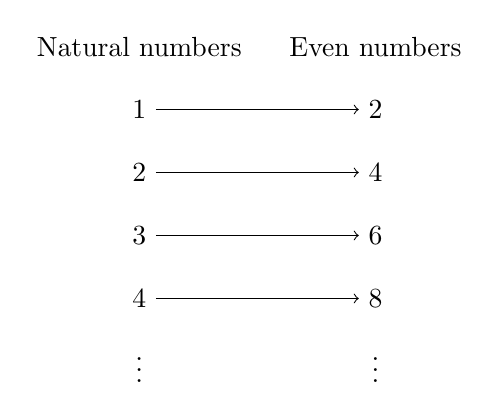
\begin{tikzpicture}
  \node (a1) at (0,3) {$1$};
  \node (a2) at (0,2.2) {$2$};
  \node (a3) at (0,1.4) {$3$};
  \node (a4) at (0,0.6) {$4$};
  \node at (0,-0.2) {$\vdots$};
  \node (b1) at (3,3) {$2$};
  \node (b2) at (3,2.2) {$4$};
  \node (b3) at (3,1.4) {$6$};
  \node (b4) at (3,0.6) {$8$};
  \node at (3,-0.2) {$\vdots$};
  \draw[->] (a1) -- (b1);
  \draw[->] (a2) -- (b2);
  \draw[->] (a3) -- (b3);
  \draw[->] (a4) -- (b4);
  \node at (0,3.8) {Natural numbers};
  \node at (3,3.8) {Even numbers};
\end{tikzpicture}
\end{center}

Pair each natural number $n$ with $2n$, as shown. Every even number is reached and every natural number has a partner. Thus the two collections have \textbf{the same size}, although evens are only part of the naturals! A part can equal the whole: infinity's first strange rule. Galileo noticed it, but it troubled mathematicians for over two centuries. Cantor finally clarified it in the late nineteenth century. Fiercely attacked by colleagues, some calling his theory a disease, he nevertheless made one-to-one correspondence the measuring stick for infinity.

He measured familiar sets. Integers, including zero and negatives, match natural numbers by listing $0, -1, 1, -2, 2, \ldots$. More surprisingly, \textbf{rational numbers also match natural numbers}. Rationals densely fill the line, infinitely many in every interval: how can they be listed? Group positive fractions by numerator-plus-denominator: sum $2$ gives $\frac{1}{1}$; sum $3$ gives $\frac{1}{2}, \frac{2}{1}$; sum $4$ gives $\frac{1}{3}, \frac{2}{2}, \frac{3}{1}$; and so on. Every fraction eventually appears and every rational receives a queue number. A set matching the naturals is \textbf{countable}: the count never ends, but everyone can queue for a number.

So far infinity seems to have one size, merely playing hide-and-seek. The real thunder comes next.

\begin{dingli}[Cantor's diagonal theorem]
The real and natural numbers do not have equal cardinality: real numbers \textbf{cannot be listed} in a single sequence. Infinity therefore has at least two sizes.
\end{dingli}

\begin{proof}
Suppose, for contradiction, that someone claims to list every real number between $0$ and $1$:
\begin{align*}
\text{Number 1:}\ & 0.\mathbf{3}\,1\,4\,1\,5\,\ldots\\
\text{Number 2:}\ & 0.2\,\mathbf{7}\,1\,8\,2\,\ldots\\
\text{Number 3:}\ & 0.1\,4\,\mathbf{1}\,4\,2\,\ldots\\
\text{Number 4:}\ & 0.5\,7\,7\,\mathbf{2}\,1\,\ldots\\
& \ \vdots
\end{align*}
Construct a new decimal $r$. Its first digit differs from the first listed number's first digit, say changing $3$ to $4$; its second differs from the second number's second digit, changing $7$ to $8$; its third changes the diagonal $1$ to $2$; its fourth changes $2$ to $3$; continue along the diagonal. The result, $r = 0.4823\ldots$, is a genuine real number between $0$ and $1$.

Is it listed? Not first, because the first digit differs; not second, because the second differs; not $n$th, because its $n$th digit differs from that of the $n$th number. Every entry mismatches in a chosen position, so \textbf{the supposedly complete list omitted it}. No proposed list escapes this construction: give any list and diagonalisation produces a missing number. The assumption is false. Reals cannot be listed; there are more of them than naturals.
\end{proof}

\begin{shuyu}{Cardinality}
\textbf{Intuition:} A set's size, measured by pairing rather than counting. Collections admitting a one-to-one correspondence have equal cardinality.

\textbf{Formal description:} The naturals' cardinality is $\aleph_0$, read "aleph-null". The larger cardinality of the reals is called the cardinality of the continuum. It can be proved that $\aleph_0$ is the smallest infinite cardinal.

\textbf{Example:} Evens, integers, and rationals have cardinality $\aleph_0$; reals, decimals between $0$ and $1$, and points on the number line have continuum cardinality.
\end{shuyu}

The diagonal number $r$ is not merely an imagined hypothetical object; its digits can be constructed. Try producing a missing number yourself.

\begin{shiyan}
Write five decimals between $0$ and $1$, each with five decimal places, in five rows. Choose random digits or borrow fragments of pi. For each number take its $i$th digit, meaning the digit at position $i$ in row $i$, and add $1$, wrapping $9$ to $0$. Assemble the five new digits into a decimal. Check that it differs from row 1 in position 1, row 2 in position 2, and so on: it is absent from the list. Repeat with new numbers. You have performed Cantor's diagonal argument, except that his list was infinite. The logic of a deliberately mismatching position is identical.
\end{shiyan}

The story continues. Cantor proved that for any set $A$, the set of all its subsets, its power set, is strictly larger than $A$. There is therefore no largest infinity, only larger ones: beyond $\aleph_0$ lies the continuum, beyond that still larger sizes, without end. Is the continuum the very next infinity after $\aleph_0$? This natural question, the continuum hypothesis, has an answer stranger than the question. We return to it later.

\section{The Barber and the Impossible Catalogue}

Different sizes of infinity are startling enough, but a deeper crack appeared in sets themselves.

Early twentieth-century mathematicians hoped sets could underpin all mathematics: numbers could be defined as sets, and figures, functions, and equations reduced to them. Secure foundations would support an eternal mathematical building. The central assumption sounded harmless: \textbf{any clearly stated condition defines the set of all things satisfying it}. Being even defines the even numbers; being red defines red things.

In 1901, Russell found a fatal condition: \textbf{not being an element of oneself}. Most sets satisfy it: the set of all apples is not itself an apple and therefore does not contain itself. Collect every such set into $R$:
\[
R = \{\, x \mid x \notin x \,\},
\]
Does $R$ contain itself? If $R \in R$, then $R$ meets the condition of not containing itself, so $R \notin R$. If $R \notin R$, then $R$ qualifies for membership in $R$, so $R \in R$. Both directions contradict themselves: \textbf{this set cannot even exist}.

The popular version is a village barber who shaves exactly those villagers who do not shave themselves. Does he shave himself? If yes, he belongs among self-shavers and must not; if no, he belongs among non-self-shavers and must. Such a barber cannot exist, not through poor skill but through a contradictory job description.

\begin{fanli}
"Every clearly stated condition defines a set" sounds unassailable, but Russell's paradox shows it can destroy the system. Another tempting mistake says that all infinities are alike and therefore offer nothing to study. Cantor's diagonal proof shows not only differences, but endlessly many levels of difference. \textbf{Intuition often stops working before infinity; that is why rigorous definitions are essential.}
\end{fanli}

Russell's paradox forced rules for sets' birth: specify exactly which sets may be constructed and how. These rules are \textbf{axioms}. The most widely used system, ZF or ZFC with the axiom of choice, roughly permits the empty set, unions of existing sets, power sets, and subsets selected from infinite sets by definite rules, among other constructions. Notice that subset selection permits choosing qualifying elements from a known set $A$, but \textbf{not} collecting all qualifying things out of nowhere. Russell's $R$ requires precisely that unrestricted collection, so it is politely excluded and the paradox dissolves.

\begin{shuyu}{Axiom}
\textbf{Intuition:} The rules of a game. Instead of asking why the rules hold, ask whether following them creates contradictions and what play they allow.

\textbf{Formal description:} An axiom is a starting statement accepted without proof; a theorem is a conclusion derived from axioms through rules of inference.

\textbf{Example:} Through an external point there is exactly one line parallel to a given line: an axiom of Euclidean geometry. Change it and obtain different geometries, as in our earlier parallel-postulate story.
\end{shuyu}

This changed mathematicians' view of axioms. Ancient Greeks treated them as self-evident truths; twentieth-century mathematicians treated them as game rules. The key questions became \textbf{consistency}, avoiding contradiction, and \textbf{fruitfulness}, yielding rich theorems. Euclidean geometry, set theory, and probability all establish rules before exploring their consequences.

\section{Godel: Mathematics Cannot Contain Every Truth}

Axiomatisation inspired a grand hope: could a sufficiently strong formal system of axioms and inference rules be \textbf{consistent}, never deriving contradictions; \textbf{complete}, proving every true natural-number statement; and able to prove its own consistency mathematically? Hilbert's programme sought a permanent certificate of mathematical safety.

In 1931, the twenty-five-year-old Godel proved two theorems refuting central parts of this plan. In very informal language:

\begin{dingli}[Godel's incompleteness theorems, informal version]
Every consistent axiomatic system that is sufficiently strong, at least expressing natural-number arithmetic, and has mechanically checkable rules contains statements \textbf{true but unprovable within that system}. Moreover, the system \textbf{cannot prove its own consistency}.
\end{dingli}

We must explain the simplification and its \textbf{limits of applicability}. These are precise theorems about formal systems, with technical assumptions. Mechanically checkable rules, for instance, mean a computer can check the axiom list item by item. The conclusion is \textbf{not} that mathematics is unreliable, \textbf{not} that nothing can be trusted, and certainly not permission to believe anything unproved. It says precisely that \textbf{provability} and \textbf{truth} cannot fully coincide in any fixed sufficiently strong rule system. Some truths require stepping outside it or adding axioms.

Godel's construction is astonishing. His encoding, now called Godel numbering, translates formulas and proofs into natural numbers. Thus the statement that proposition $P$ is provable becomes an arithmetic statement: the system discusses its own proofs. Echoing the liar paradox, he constructs an arithmetic statement $G$ meaning "$G$ is not provable in this system". If the system proves $G$, it proves a falsehood, contradicting consistency. Hence, assuming consistency, $G$ is indeed unprovable; but that is exactly what $G$ says, so $G$ is true. That produces truth without proof. Remember our map inside a map? Taming self-reference creates mathematics' sharpest breakthroughs.

\begin{lianjie}
Godel's idea of encoding symbol strings as numbers so systems can discuss themselves changed the world in another form fifty years later. Programmes are fundamentally numbers too, since code is a symbol string; programmes analyse other programmes and themselves. Turing's proof that no universal programme decides all halting questions uses the same diagonal self-reference. The continuum hypothesis belongs to this family too: mathematicians proved it \textbf{neither provable nor refutable} in ZFC. Godel's inaccessible truths are not an abstract threat: concrete important questions enter the blind spot. Infinity, self-reference, and computability, apparently unrelated at our opening, are three knots in one deep net.
\end{lianjie}

What does this mean for us? Honestly, mathematics is not a final-answer stamping machine, but a territory with ever-new frontiers. Each solved question exposes new blank spaces at the map's edge. This is not failure, but evidence that mathematics remains alive.

\begin{toolbox}
New tools from this chapter:
\begin{itemize}
\item \textbf{One-to-one correspondence}: Compare set sizes, even infinite ones, without counting to the end.
\item \textbf{Diagonalisation}: Alter the $n$th feature of the $n$th object to create something outside a list, proving uncountability and powering self-reference.
\item \textbf{Axiomatic thinking}: View theories as rules plus deduction, valuing consistency and richness rather than self-evidence.
\item \textbf{A meta-level viewpoint}: Step outside a system to study it. Questions of what can be proved, computed, or completely mapped often become clear only one level up.
\end{itemize}
\end{toolbox}

\section{Six Lenses: One Map of the Whole Book}

After twenty chapters, it is time to map our travels. Six overlapping, mutually illuminating lenses offer views of mathematics:

\begin{center}
\begin{tabular}{lll}
\toprule
Lens & Central questions & An unresolved conjecture \\
\midrule
Number & \shortstack[l]{Counting, measurement,\\exact representation} & \shortstack[l]{Riemann hypothesis: fine\\prime-distribution patterns}\\
Shape & \shortstack[l]{Position, shape,\\distance, symmetry} & \shortstack[l]{Optimal sphere packing in\\most higher dimensions}\\
Change & \shortstack[l]{Rates, accumulation,\\limits} & \shortstack[l]{Smoothness of\\Navier--Stokes solutions}\\
Structure & \shortstack[l]{Relations, operations,\\patterns themselves} & \shortstack[l]{$P$ versus $NP$: is checking\\always easier than solving?}\\
Randomness & \shortstack[l]{Regularity within\\uncertainty} & \shortstack[l]{Many questions between\\random processes and chaos}\\
Proof & Grounds for belief & \shortstack[l]{How far machine proof can go:\\an open question}\\
\bottomrule
\end{tabular}
\end{center}

\textbf{Number} was our starting point. From tally knots to fractions, negatives, irrationals, and imaginary numbers, every surprised "That counts as a number too?" expanded the territory. Now even infinities receive classifications and numbers.

\textbf{Shape} led from Pythagoras to symmetry, transformations, and non-Euclidean geometry. It is not merely drawing, but turning positional relationships into computable objects.

\textbf{Change} leaps from static quantities to processes: speed, slope, and area transform into one another, differentiation and integration become inverse operations, and mathematics captures motion on paper.

\textbf{Structure} is the most abstract and modern lens. Addition, rotation, permutation, and matrices look unrelated yet share operational patterns. Groups, graphs, and vector spaces study relations between relations.

\textbf{Randomness} accepts unavoidable chance, then asks what necessity hides inside it. Large numbers, expectations, and statistical inference support definite decisions under uncertainty.

\textbf{Proof} binds the other five lenses and runs through the book: from apparently true to why true, from inductive guesses to deductive chains. Here we pushed that thread to its end. Proof itself can be studied, and it has boundaries.

These lenses are not islands. The next question shows them meeting in one landscape.

\section{One Question, Three Paths: The Shortest Route}

Consider an old puzzle. An ant must crawl from vertex $A$ to the opposite vertex $B$ of a cube-shaped cardboard box, staying on its surface. How long is the shortest route?

\textbf{First approach, through shape: unfolding.} Cut along cube edges and flatten the surface. Surface routes become planar lines, where a straight segment is shortest. For cube side $1$, unfold two adjacent faces into a $2 \times 1$ rectangle. The distance from $A$ to $B$ is $\sqrt{2^2 + 1^2} = \sqrt{5}$. A transformation translates a difficult surface question into an easy planar one. Geometry often gains power not by harder calculation but by \textbf{changing the space we look in}.

\textbf{Second approach, through structure: graphs and greed.} Modify the question: a city has junctions and known road lengths; find the shortest home-to-school route. Draw junctions as vertices and roads as weighted edges, forming a \textbf{graph}. An elegant greedy strategy keeps the currently known distances from home, repeatedly \textbf{fixing} the nearest junction, since detouring through another cannot reach it sooner, then updating its neighbours. When school is fixed, its shortest distance is known. Dijkstra's algorithm is one heart of navigation software, relying not on geometric intuition but on extracting distance structure step by step.

\begin{center}
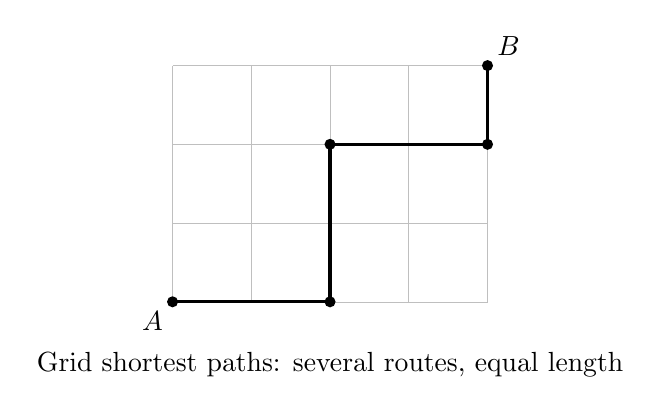
\begin{tikzpicture}
  \draw[step=1,gray!50,very thin] (0,0) grid (4,3);
  \draw[very thick] (0,0) -- (2,0) -- (2,2) -- (4,2) -- (4,3);
  \fill (0,0) circle (2pt) node[below left] {$A$};
  \fill (4,3) circle (2pt) node[above right] {$B$};
  \foreach \p in {(2,0),(2,2),(4,2)} \fill \p circle (2pt);
  \node at (2,-0.8) {Grid shortest paths: several routes, equal length};
\end{tikzpicture}
\end{center}

\textbf{Third approach, through change: let nature calculate.} Modify it again. Light bends entering water from air, choosing an angle that \textbf{minimises total travel time}: Fermat's least-time principle. Deriving refraction needs no account of what light thinks; write travel time as a function of path and ask when small changes cease to reduce it. Calculus and the calculus of variations optimise among \textbf{infinitely many possible paths}, not a finite shortlist. Many physical laws, including least action, share this form.

One shortest-path idea, three spirits: geometry transforms, algorithms exploit structure, and analysis optimises among infinitely many candidates. They translate and inspire one another: navigation contains discretised geometry; variational problems contain continuous versions of greedy reasoning. A unified mathematical map does not merge every subject into one course. It recognises that \textbf{every ascent of the same mountain meets at its summit}. Prime distribution likewise belongs to number through sieves and factors, to shape through strange diagonal patterns in prime spirals, to randomness through lottery-like large-scale behaviour, and to change through the logarithmic density of the prime number theorem. Deep questions never belong to just one lens.

\begin{pandeng}
Further keywords: \textbf{set theory}, arithmetic of infinity; \textbf{mathematical logic}, mathematics of proof; \textbf{halting problem}, computation's boundaries; \textbf{graph theory}, shortest paths and network flows; \textbf{calculus of variations}, optimisation among infinite choices; and \textbf{Riemann hypothesis}, the million-dollar prime mystery. Each opens another book.
\end{pandeng}

\section*{Questions to Think About}

\textbf{Observation}

1. Following the correspondence between evens and naturals, construct one between odd numbers and all integers, including negatives. \emph{Hint: list integers as $0, 1, -1, 2, -2, \ldots$, then match them with the odd-number queue.}

2. The cube can be unfolded in different ways. Draw another net, calculate its route length, and compare with $\sqrt{5}$. \emph{Hint: locate $A$ and $B$ on the unfolded grid. Some unfoldings give $\sqrt{5}$, others longer distances; the shortest wins.}

\textbf{Proof}

3. Prove that the reals between $0$ and $1$ are as numerous as all reals. \emph{Hint: find a one-to-one correspondence stretching a finite interval onto the line. Start with the graph of $y = \tan x$ and explain its one-to-one property.}

4. Use diagonal reasoning to show that there is no set of all sets. \emph{Hint: if such a set $U$ existed, the power set of $U$ should be no larger than $U$, but Cantor proved the power set strictly larger.}

\textbf{Challenge}

5. The barber paradox is resolved by saying no such barber exists. Someone changes the rule: "I shave everyone who does not shave themselves, except me." Does the paradox vanish? Are there other difficulties? \emph{Hint: the new rule is consistent, but who is omitted among non-self-shavers, and who tends the barber's beard? Compare ZF's restriction to selecting subsets from an existing set.}

6. Godel's statement $G$ says it is unprovable. Why not add $G$ as an axiom and make the system complete? Why is this not a permanent solution? \emph{Hint: the new system remains sufficiently strong and consistent if the original was, so the theorem applies again.}

\section*{The Door to the Next Chapter}

This book has no next chapter. Yours is just beginning.

If the book is a map, the edges marked "Here be dragons" point towards your real destinations. Here are signposts for travellers with different tastes.

If you enjoy \textbf{competitions}, they squeeze every drop from school mathematics: combinatorics, number theory, geometry, and inequalities teach ingenious moves with minimal resources. Their essence is depth, not speed. Finding three solutions to one problem takes you farther than grinding through three hundred problems.

If you enjoy \textbf{programming}, you already hold the book's handiest laboratory. Test a hundred million Goldbach examples, simulate the law of large numbers, or implement Dijkstra in a maze solver. Mathematics gives vision and code gives brute force; together they almost feel like cheating.

If you enjoy \textbf{modelling}, the real world has been waiting: why epidemic curves bend as they do, how delivery riders should route themselves, or why a song sounds pleasing. Modelling translates tangled reality into one of our six lenses. Wrong translations are nothing to fear; errors teach better ones.

If you head towards \textbf{university mathematics}, you will meet the full versions of these stories. Calculus becomes analysis, geometry becomes topology and manifolds, randomness becomes measure theory, and axioms, diagonals, and incompleteness become mathematical logic. Behind every informal explanation here, you will discover a genuine proof.

If you continue from \textbf{pure curiosity}, congratulations: you have the best reason. Many great advances began with a useless "What if?" Nobody knew Cantor's questions about infinity would help underpin computer science; prime-number players never imagined their games guarding the world's banking passwords.

How did the art teacher resolve the campus map? Reportedly, she drew a tiny map in its corner, placed a nearly invisible dot inside that, and stopped. Beside it she wrote: "For anything smaller, go into the campus and look for yourself."

Mathematics is like that. No map, however detailed, replaces walking. We have lit the spark; the road ahead is yours to illuminate.
